%File: anonymous-submission-latex-2025.tex
\documentclass[letterpaper]{article} % DO NOT CHANGE THIS
\usepackage[submission]{aaai25}  % DO NOT CHANGE THIS
\usepackage{times}  % DO NOT CHANGE THIS
\usepackage{helvet}  % DO NOT CHANGE THIS
\usepackage{courier}  % DO NOT CHANGE THIS
\usepackage[hyphens]{url}  % DO NOT CHANGE THIS
\usepackage{graphicx} % DO NOT CHANGE THIS
\urlstyle{rm} % DO NOT CHANGE THIS
\def\UrlFont{\rm}  % DO NOT CHANGE THIS
\usepackage{natbib}  % DO NOT CHANGE THIS AND DO NOT ADD ANY OPTIONS TO IT
\usepackage{caption} % DO NOT CHANGE THIS AND DO NOT ADD ANY OPTIONS TO IT
\frenchspacing  % DO NOT CHANGE THIS
\setlength{\pdfpagewidth}{8.5in} % DO NOT CHANGE THIS
\setlength{\pdfpageheight}{11in} % DO NOT CHANGE THIS
%
% These are recommended to typeset algorithms but not required. See the subsubsection on algorithms. Remove them if you don't have algorithms in your paper.
\usepackage{algorithm}
\usepackage{algorithmic}

%
% These are are recommended to typeset listings but not required. See the subsubsection on listing. Remove this block if you don't have listings in your paper.
\usepackage{newfloat}
\usepackage{listings}
\DeclareCaptionStyle{ruled}{labelfont=normalfont,labelsep=colon,strut=off} % DO NOT CHANGE THIS
\lstset{%
	basicstyle={\footnotesize\ttfamily},% footnotesize acceptable for monospace
	numbers=left,numberstyle=\footnotesize,xleftmargin=2em,% show line numbers, remove this entire line if you don't want the numbers.
	aboveskip=0pt,belowskip=0pt,%
	showstringspaces=false,tabsize=2,breaklines=true}
\floatstyle{ruled}
\newfloat{listing}{tb}{lst}{}
\floatname{listing}{Listing}
%
% Keep the \pdfinfo as shown here. There's no need
% for you to add the /Title and /Author tags.
\pdfinfo{
/TemplateVersion (2025.1)
}

\usepackage{amsmath}
\usepackage{array}
\usepackage{multirow}
\usepackage{booktabs}
\usepackage{diagbox}
\usepackage[table]{xcolor}
\usepackage{hhline}
\usepackage{appendix}

% DISALLOWED PACKAGES
% \usepackage{authblk} -- This package is specifically forbidden
% \usepackage{balance} -- This package is specifically forbidden
% \usepackage{color (if used in text)
% \usepackage{CJK} -- This package is specifically forbidden
% \usepackage{float} -- This package is specifically forbidden
% \usepackage{flushend} -- This package is specifically forbidden
% \usepackage{fontenc} -- This package is specifically forbidden
% \usepackage{fullpage} -- This package is specifically forbidden
% \usepackage{geometry} -- This package is specifically forbidden
% \usepackage{grffile} -- This package is specifically forbidden
% \usepackage{hyperref} -- This package is specifically forbidden
% \usepackage{navigator} -- This package is specifically forbidden
% (or any other package that embeds links such as navigator or hyperref)
% \indentfirst} -- This package is specifically forbidden
% \layout} -- This package is specifically forbidden
% \multicol} -- This package is specifically forbidden
% \nameref} -- This package is specifically forbidden
% \usepackage{savetrees} -- This package is specifically forbidden
% \usepackage{setspace} -- This package is specifically forbidden
% \usepackage{stfloats} -- This package is specifically forbidden
% \usepackage{tabu} -- This package is specifically forbidden
% \usepackage{titlesec} -- This package is specifically forbidden
% \usepackage{tocbibind} -- This package is specifically forbidden
% \usepackage{ulem} -- This package is specifically forbidden
% \usepackage{wrapfig} -- This package is specifically forbidden
% DISALLOWED COMMANDS
% \nocopyright -- Your paper will not be published if you use this command
% \addtolength -- This command may not be used
% \balance -- This command may not be used
% \baselinestretch -- Your paper will not be published if you use this command
% \clearpage -- No page breaks of any kind may be used for the final version of your paper
% \columnsep -- This command may not be used
% \newpage -- No page breaks of any kind may be used for the final version of your paper
% \pagebreak -- No page breaks of any kind may be used for the final version of your paperr
% \pagestyle -- This command may not be used
% \tiny -- This is not an acceptable font size.
% \vspace{- -- No negative value may be used in proximity of a caption, figure, table, section, subsection, subsubsection, or reference
% \vskip{- -- No negative value may be used to alter spacing above or below a caption, figure, table, section, subsection, subsubsection, or reference

\setcounter{secnumdepth}{0} %May be changed to 1 or 2 if section numbers are desired.

% The file aaai25.sty is the style file for AAAI Press
% proceedings, working notes, and technical reports.
%

% Title

% Your title must be in mixed case, not sentence case.
% That means all verbs (including short verbs like be, is, using,and go),
% nouns, adverbs, adjectives should be capitalized, including both words in hyphenated terms, while
% articles, conjunctions, and prepositions are lower case unless they
% directly follow a colon or long dash
\title{From Persona to Person: Enhancing the Naturalness with Multiple Discourse Relations Graph Learning in Personalized Dialogue Generation}
\author{
    %Authors
    % All authors must be in the same font size and format.
    Chih-Hao Hsu, \\
    Hung-Yu Kao
}
\affiliations{
    %Afiliations
    \textsuperscript{\rm 1}Association for the Advancement of Artificial Intelligence\\
    % If you have multiple authors and multiple affiliations
    % use superscripts in text and roman font to identify them.
    % For example,

    % Sunil Issar\textsuperscript{\rm 2},
    % J. Scott Penberthy\textsuperscript{\rm 3},
    % George Ferguson\textsuperscript{\rm 4},
    % Hans Guesgen\textsuperscript{\rm 5}
    % Note that the comma should be placed after the superscript

    1101 Pennsylvania Ave, NW Suite 300\\
    Washington, DC 20004 USA\\
    % email address must be in roman text type, not monospace or sans serif
    proceedings-questions@aaai.org
%
% See more examples next
}

%Example, Single Author, ->> remove \iffalse,\fi and place them surrounding AAAI title to use it
\iffalse
\title{My Publication Title --- Single Author}
\author {
    Author Name
}
\affiliations{
    Affiliation\\
    Affiliation Line 2\\
    name@example.com
}
\fi

\iffalse
%Example, Multiple Authors, ->> remove \iffalse,\fi and place them surrounding AAAI title to use it
\title{My Publication Title --- Multiple Authors}
\author {
    % Authors
    First Author Name\textsuperscript{\rm 1},
    Second Author Name\textsuperscript{\rm 2},
    Third Author Name\textsuperscript{\rm 1}
}
\affiliations {
    % Affiliations
    \textsuperscript{\rm 1}Affiliation 1\\
    \textsuperscript{\rm 2}Affiliation 2\\
    firstAuthor@affiliation1.com, secondAuthor@affilation2.com, thirdAuthor@affiliation1.com
}
\fi


% REMOVE THIS: bibentry
% This is only needed to show inline citations in the guidelines document. You should not need it and can safely delete it.
\usepackage{bibentry}
% END REMOVE bibentry

\begin{document}

\maketitle

\appendix
\section{Appendix}

\subsection{Coherence Relations Annotation} \label{sec:coherence_reltaions_annotation}
To facilitate the model's understanding of how two sentences in a conversation are effectively connected, we employ Large Language Models (LLMs) such as GPT-4, Mixtral-8x7b, and LLaMA-3 to assist in annotating coherence relations. There are, in total, 16 discourse relations according to STAC \cite{asher-etal-2016-discourse}, namely, \textbf{comment}, \textbf{clarification-question}, \textbf{elaboration}, \textbf{acknowledgment}, \textbf{continuation}, \textbf{explanation}, \textbf{conditional}, \textbf{question-answer}, \textbf{alternation}, \textbf{question-elaboration}, \textbf{result}, \textbf{background}, \textbf{narration}, \textbf{correction}, \textbf{parallel} and \textbf{contrast}. On top of these relationships, we add \textbf{topic-shift} to represent coherent topic transitions between conversations. 

Each pair of utterances could be annotated with zero to three different relations. In total, we have annotated 1,942,177 pairs of utterances for their coherence relations. An example of annotated results can be seen in Table \ref{table:coherence-relations-annotated-example}. The prompt for coherence relations annotations is shown in Figure \ref{fig:coherence_reltaions_annotated_prompt}

\begin{table*}[h]
\centering
\def\arraystretch{1.4}%
\begin{tabular}{|c|l|c|}
\hline

\rowcolor[RGB]{204,217,245}
\textbf{Index} & \multicolumn{2}{|c|}{\textbf{Dialogue}} \\
\hline

0 & \multicolumn{2}{|p{14cm}|}{[PERSON 1:] Hello what are doing today?} \\
\cline{1-1}
1 & \multicolumn{2}{|p{14cm}|}{[PERSON 2:] I am good, I just got off work and tired, I have two jobs.} \\
\cline{1-1}
2 & \multicolumn{2}{|p{14cm}|}{[PERSON 1:] I just got done watching a horror movie.} \\
\cline{1-1}
3 & \multicolumn{2}{|p{14cm}|}{[PERSON 2:] Wow! I do love a good horror movie. Loving this cooler weather.} \\
\cline{1-1}
4 & \multicolumn{2}{|p{14cm}|}{[PERSON 1:] But a good movie is always good.} \\
\cline{1-1}
5 & \multicolumn{2}{|p{14cm}|}{...} \\
\hline

\rowcolor[RGB]{204,217,245}
\textbf{Index} & \multicolumn{1}{|c|}{\textbf{Utterance}} & \textbf{Coherence Relations} \\
\hline

0 & Hello what are doing today? & \multirow{2}{*}{QA, Explanation} \\
\cline{1-2}
1 & I am good, I just got off work and tired, I have two jobs. & \\
\hline

0 & Hello what are doing today? & \multirow{2}{*}{QA} \\
\cline{1-2}
2 & I just got done watching a horror movie. & \\

\hline
\multicolumn{3}{|c|}{...} \\
\hline

1 & I am good, I just got off work and tired, I have two jobs. & \multirow{2}{*}{Topic Shift} \\
\cline{1-2}
2 & I just got done watching a horror movie. & \\
\hline

\multicolumn{3}{|c|}{...} \\
\hline

\end{tabular}
\caption{Examples of coherence relations annotated by the LLaMA-3-70B\protect\footnotemark\cite{llama3modelcard}. We annotated all utterance pairs in the dialogue, and the examples shown here represent only a subset of the complete dataset.}
\label{table:coherence-relations-annotated-example}
\end{table*}
\footnotetext{https://huggingface.co/meta-llama/Meta-Llama-3-70B-Instruct}

\begin{figure}[ht]
    \centering
    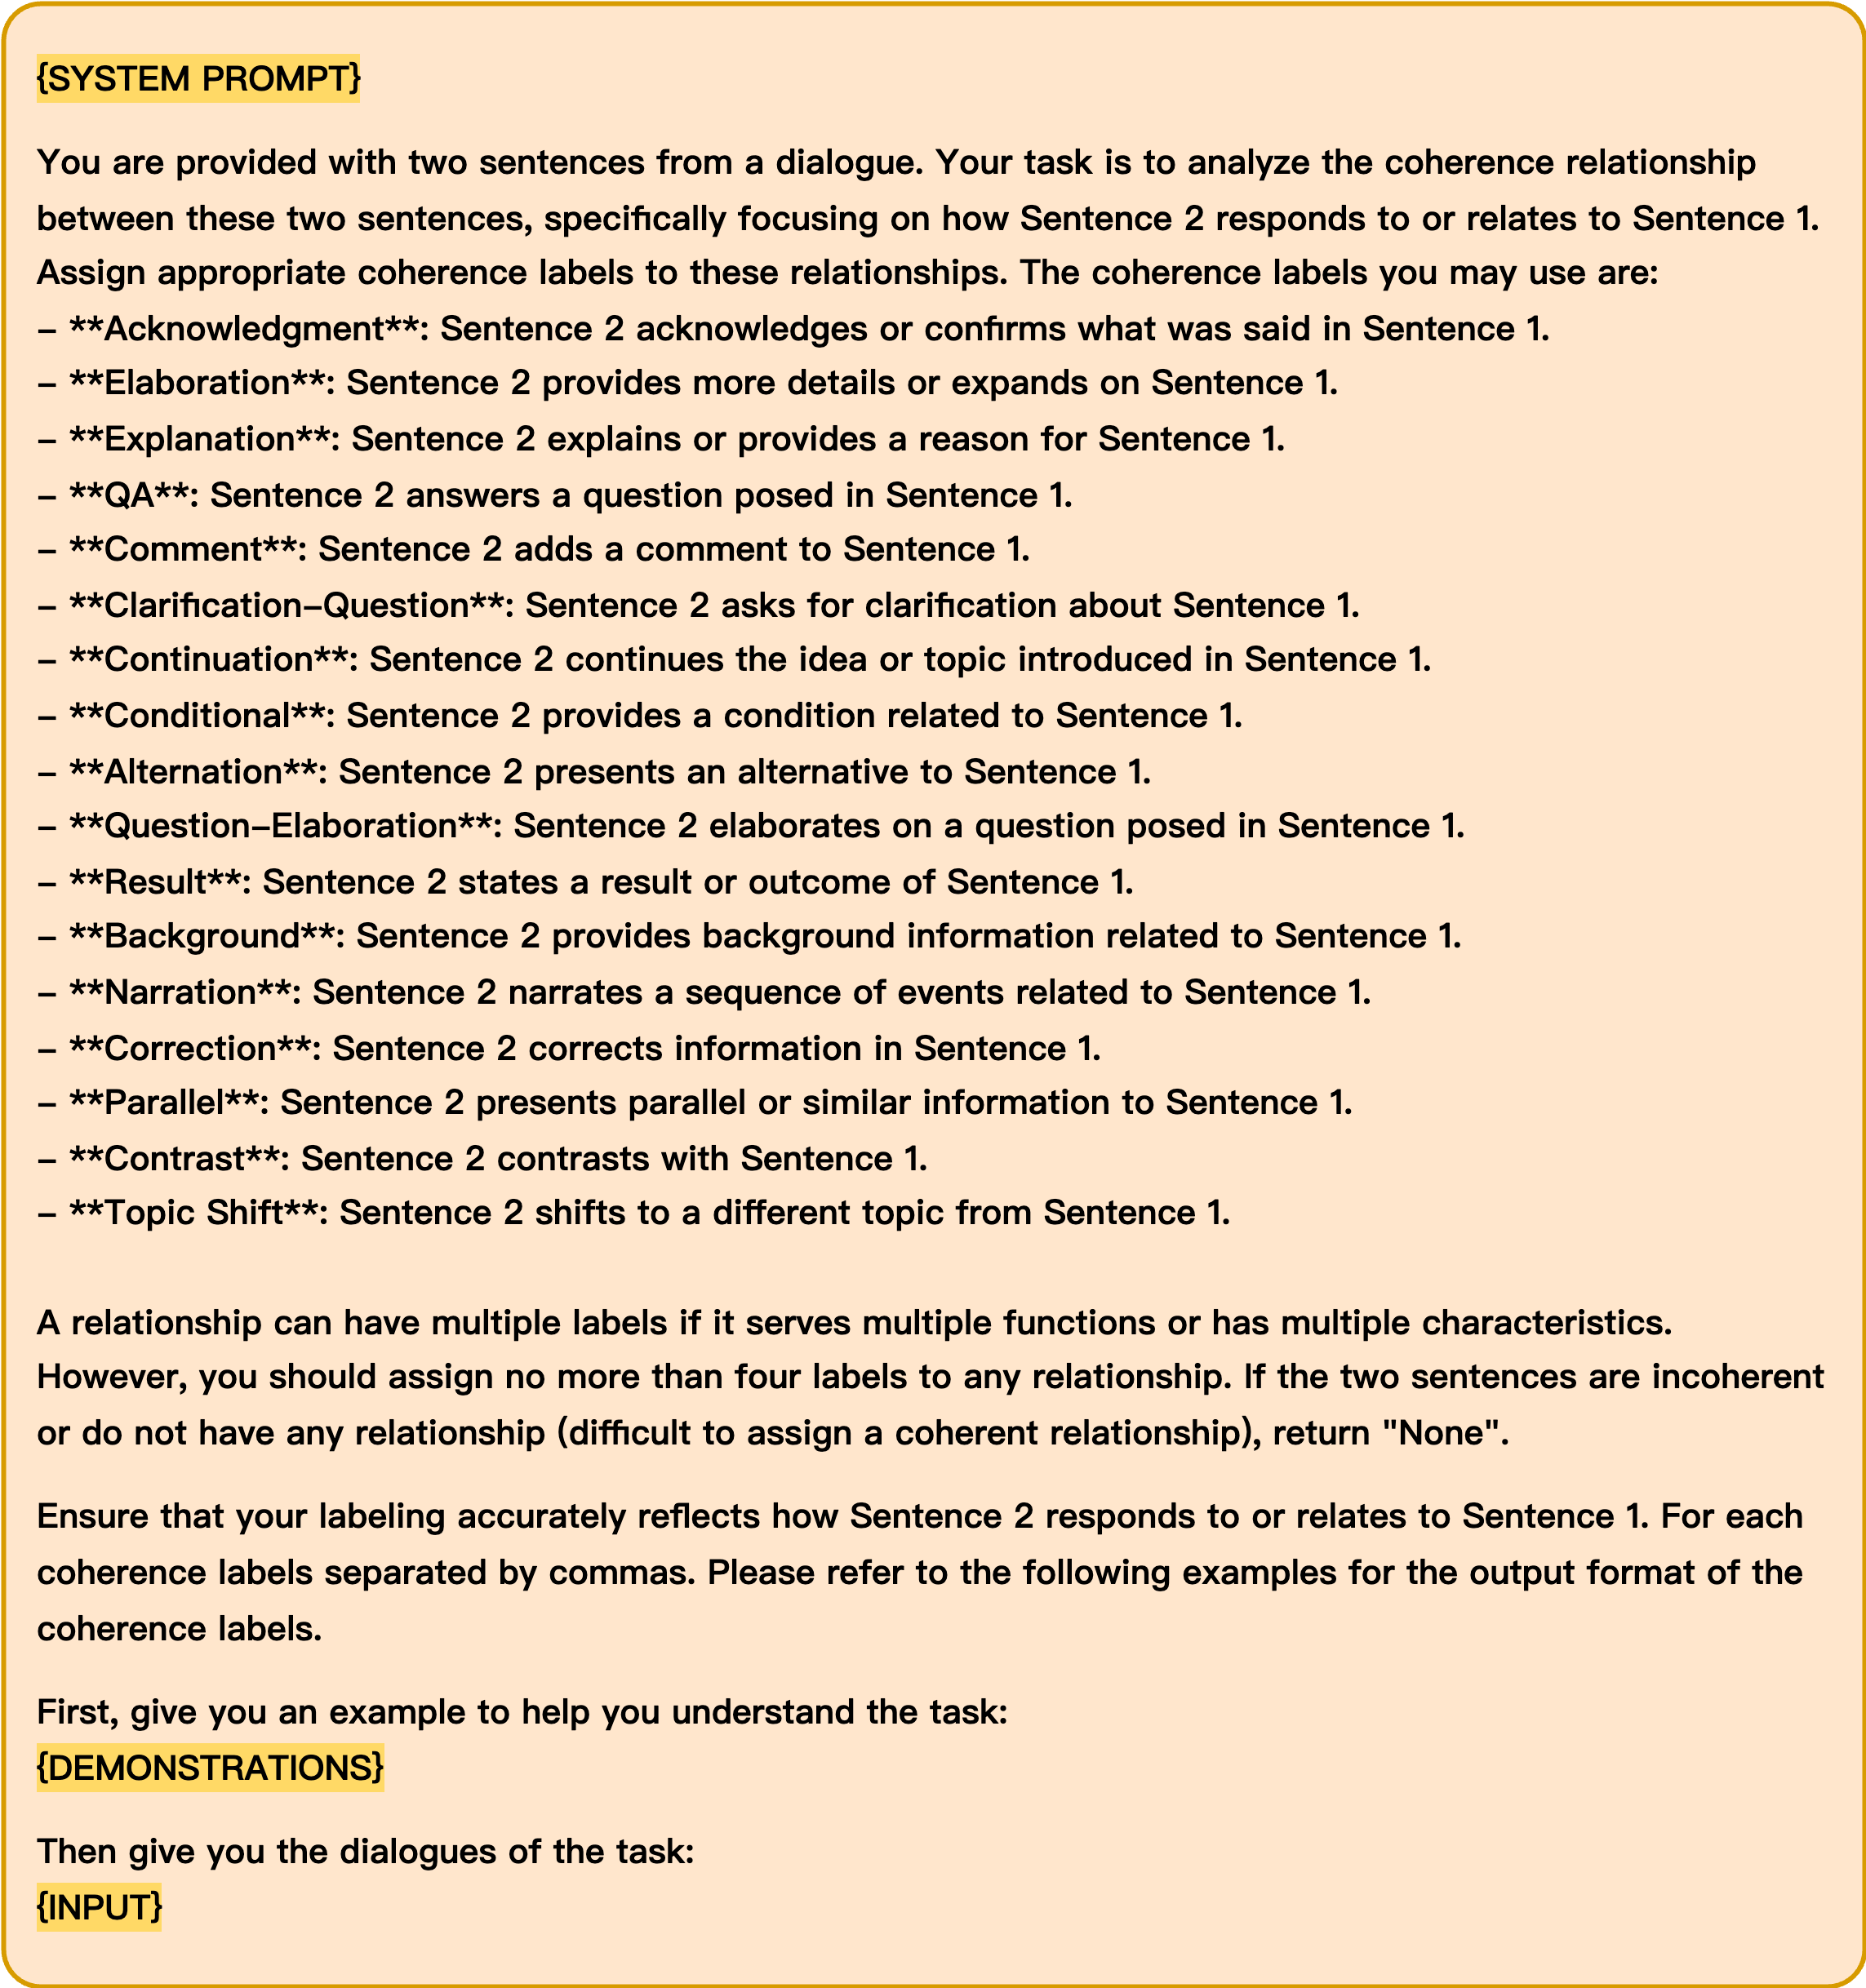
\includegraphics[width=0.5\textwidth]{./images/coherence_reltaions_annotated_prompt.png}
    \caption{The prompt of Coherence Relations Annotation.}
    \label{fig:coherence_reltaions_annotated_prompt}
\end{figure}

\subsection{Implementation Details}
The \textbf{MUDI} is mainly implemented in PyTorch. Our backbone Generator is BART-large\footnote[2]{https://huggingface.co/facebook/bart-large}. For Generator training, we train it using a batch size of 4 on 1 NVIDIA A100 80GB
GPU via the AdamW optimizer with a learning rate of \(5 \times 10^{-6}\) and a
weight decay of 0.01. For the Dialogue Graph Encoder training, it is conducted on a single NVIDIA RTX 4090 GPU using a batch size of 512. The training also employs the AdamW optimizer, but with a learning rate of \(2 \times 10^{-5}\) and the same weight decay of 0.01. In the Dialogue Graph Encoder, we initially employ the SBERT model "all-mpnet-base-v2"\footnote[3]{https://huggingface.co/sentence-transformers/all-mpnet-base-v2} to encode both the utterances and persona sentences, thereby initializing the node embeddings. We construct the Dialogue Graph by keeping the 3-hop neighbors. The model employs a 2-layer GNN with 4 multi-heads and a hidden dimension of 512. The weights for the different tasks are as follows: the weight of the Coherence Relation Classification task is 1.5, the weight of both types of Next Response Type Prediction tasks is 1.5, and the weight of the Link Prediction task is 1.2. For training the generator, we retain the most recent 5 turns of dialogue as historical context and choose the top-3 predicted response types for the prompt. We set \(\tau = 0.2\) for the Dynamic Weighted Aggregation.

% ----------------------------------------------
% Table 1: Text Similarity
% ----------------------------------------------

\begin{table*}
\centering
\def\arraystretch{1.3}%
\begin{tabular}{|c|c|c|c|c|c|c|}
\hline
\multicolumn{2}{|c|}{\multirow{2}{*}{\textbf{Model}}}  & \multicolumn{5}{c|}{\textbf{Text Similarity}} \\
\cline{3-7}

\multicolumn{2}{|c|}{} & BLEU-1 $\uparrow$ & BLEU-2 $\uparrow$ & ROUGE-1 $\uparrow$ & ROUGE-L $\uparrow$ & BERTScore $\uparrow$ \\
\hhline{|=======|}

\rowcolor[RGB]{242,164,100}
\multicolumn{7}{|c|}{\textbf{Large Language Model (Prompting)}} \\
\hhline{|=======|}

\multicolumn{2}{|c|}{\textbf{GPT-4}} &7.47 &2.40 &13.52 &11.06 &84.05 \\ 
\hhline{|=======|}

\rowcolor{yellow}
\multicolumn{7}{|c|}{\textbf{General Dialogue Generation}} \\
\hhline{|=======|}

\multicolumn{2}{|c|}{\textbf{DialoGPT}} &7.34	&1.54 &9.46 &8.41 &83.31 \\ 
\hline

\multirow{2}{*}{\textbf{PLATO}} & w/ persona &4.35	&1.01 &4.88 &4.80 &82.77 \\ 
\cline{2-7}

\multirow{2}{*}{\textbf{}} & w/o persona  &6.82 &1.86 &4.99 &4.77 &81.44 \\ 
\hhline{|=======|}

\rowcolor[RGB]{204,217,245}
\multicolumn{7}{|c|}{\textbf{Persona-based Dialogue Generation}} \\
\hhline{|=======|}

\multicolumn{2}{|c|}{\textbf{BoB}} &15.30 &5.39 &13.21 &12.48 &83.77 \\ 
\hline

% \multicolumn{2}{|c|}{\textbf{P$^{2}$BOT}} &- &- &- &- &- \\ 
% \hline

\multicolumn{2}{|c|}{\textbf{LMEDR}}		&15.47	&5.83	&13.28	&12.26	&85.00 \\ 
\hline

\multicolumn{2}{|c|}{\textbf{PAA}}          &\underline{16.55}    &6.28    &13.53 
&12.68    &84.42   \\
\hline

\multirow{3}{*}{\textbf{\begin{tabular}{@{}c@{}}MUDI \\ (ours)\end{tabular}}} &SP\textsubscript{$\tau=0.2$}	&15.14	&6.43	&14.87	&13.87	&85.07	\\
\cline{2-7}

\multirow{3}{*}{} &Emb\textsubscript{$\tau=0.2$}   &\underline{16.55}    &\underline{7.34}	&\textbf{\textcolor{red}{17.10}}	&\textbf{\textcolor{red}{16.13}}	&\underline{85.42}	\\
\cline{2-7}

\multirow{3}{*}{} &SP+Emb\textsubscript{$\tau=0.2$}   &\textbf{\textcolor{red}{18.19}} &\textbf{\textcolor{red}{7.77}}	&\underline{16.59}	&\underline{15.46}	&\textbf{\textcolor{red}{85.53}} \\
\hline
\end{tabular}
\caption{Automatic evaluation results on ConvAI2 dataset over our implemented approach. The best results in each column are in bold, while the second is underlined.}
\label{table:text-similarity}
\end{table*}

% ----------------------------------------------
% Table 2: Diversity
% ----------------------------------------------

\begin{table}[h]
\centering
\def\arraystretch{1.3}%
\begin{tabular}{|c|c|c|c|c|}
\hline
\multicolumn{2}{|c|}{\multirow{2}{*}{\textbf{Model}}}  &\multicolumn{3}{c|}{\textbf{Diversity}}\\
\cline{3-5}

\multicolumn{2}{|c|}{} &Ent-1 $\uparrow$ &Dist-1 $\uparrow$ &USR $\uparrow$ \\
\hhline{|=====|}

\rowcolor[RGB]{242,164,100}
\multicolumn{5}{|c|}{\textbf{Large Language Model (Prompting)}} \\
\hhline{|=====|}

\multicolumn{2}{|c|}{\textbf{GPT-4}} &9.40 &16.09 &1.00 \\ 
\hhline{|=====|}

\rowcolor{yellow}
\multicolumn{5}{|c|}{\textbf{General Dialogue Generation}} \\
\hhline{|=====|}

\multicolumn{2}{|c|}{\textbf{DialoGPT}} &\textbf{\textcolor{red}{9.05}} &36.84 &\underline{0.99} \\ 
\hline

\multirow{2}{*}{\textbf{PLATO}} & w/ persona &4.67 &\textbf{\textcolor{red}{58.18}} &0.61 \\ 
\cline{2-5}

\multirow{2}{*}{\textbf{}} & w/o persona &6.73 &43.34 &0.85 \\ 
\hhline{|=====|}

\rowcolor[RGB]{204,217,245}
\multicolumn{5}{|c|}{\textbf{Persona-based Dialogue Generation}} \\
\hhline{|=====|}


\multicolumn{2}{|c|}{\textbf{BoB}} &7.89 &41.75 &\underline{0.99} \\ 
\hline

% \multicolumn{2}{|c|}{\textbf{P$^{2}$BOT}} &- &- &- \\ 
% \hline

\multicolumn{2}{|c|}{\textbf{LMEDR}}  &7.14	&43.08	&0.94\\ 
\hline

\multicolumn{2}{|c|}{\textbf{PAA}}    &6.66	&40.27  &0.87 \\
\hline

\multirow{3}{*}{\textbf{\begin{tabular}{@{}c@{}}MUDI \\ (ours)\end{tabular}}} &SP\textsubscript{$\tau=0.2$}	&\underline{8.13}		&46.76	&\textbf{\textcolor{red}{1.00}}\\
\cline{2-5}

\multirow{3}{*}{} &Emb\textsubscript{$\tau=0.2$}   &7.65	&\underline{51.03}	&\textbf{\textcolor{red}{1.00}}\\
\cline{2-5}

\multirow{3}{*}{} &SP+Emb\textsubscript{$\tau=0.2$} 	&7.66	&47.68  &\textbf{\textcolor{red}{1.00}}\\
\hline
\end{tabular}
\caption{Automatic evaluation results for diversity tested on ConvAI2 dataset over our implemented approach. The best results in each column are in bold, while the second is underlined.}
\label{table:text-diversity}
\end{table}

% ----------------------------------------------
% Table 3: Coherence 
% ----------------------------------------------

\begin{table*}[h]
\centering
\def\arraystretch{1.3}%
\begin{tabular}{|c|c|c|c|c|}
\hline
\multicolumn{2}{|c|}{\multirow{2}{*}{\textbf{Model}}}  & \multicolumn{3}{c|}{\textbf{Coherence}} \\
\cline{3-5}

\multicolumn{2}{|c|}{} & QuantiDCE $\uparrow$ & DEAM $\uparrow$ & BARTScore$_{q \rightarrow r, c \rightarrow r}$ $\downarrow$ \\
\hline

\multicolumn{2}{|c|}{\textbf{GOLD}}          &3.19 / 2.83    &0.64 / 0.85    &5.74 / 5.70   \\
\hhline{|=====|}

\rowcolor[RGB]{242,164,100}
\multicolumn{5}{|c|}{\textbf{Large Language Model (Prompting)}} \\
\hhline{|=====|}

\multicolumn{2}{|c|}{\textbf{GPT-4}} &3.41 / 2.92 &0.87 / 0.96 &4.24 / 3.73 \\ 
\hhline{|=====|}

\rowcolor{yellow}
\multicolumn{5}{|c|}{\textbf{General Dialogue Generation}} \\
\hhline{|=====|}

\multicolumn{2}{|c|}{\textbf{DialoGPT}} &\textbf{\textcolor{red}{3.23}} / 2.79 &\textbf{\textcolor{red}{0.70}} / \textbf{\textcolor{red}{0.88}} &5.12 / 5.19 \\ 
\hline

% \multirow{2}{*}{\textbf{PLATO}} & w/ persona &3.32 / 3.43	&0.22 / 0.75 &6.42 / 6.63 \\ 
\multirow{2}{*}{\textbf{PLATO}} & w/ persona &1.68 / 1.57	&0.22 / 0.75 &6.42 / 6.63 \\ 
\cline{2-5}

\multirow{2}{*}{\textbf{}} & w/o persona  &1.87 / 1.77 &0.25 / 0.74 &5.83 / 5.80 \\ 
\hhline{|=====|}

\rowcolor[RGB]{204,217,245}
\multicolumn{5}{|c|}{\textbf{Persona-based Dialogue Generation}} \\
\hhline{|=====|}

\multicolumn{2}{|c|}{\textbf{BoB}} &2.99 / 2.76 &0.39 / 0.86 &5.82 / 5.92 \\ 
\hline

% \multicolumn{2}{|c|}{\textbf{P$^{2}$BOT}} &- &- &- \\ 
% \hline

\multicolumn{2}{|c|}{\textbf{LMEDR}}		&2.89 / 2.90	&0.43 / 0.78	&5.32 / 4.99  \\ 
\hline

\multicolumn{2}{|c|}{\textbf{PAA}}           &2.70 / \underline{2.93}    &0.56 / 0.83    &5.17 / \underline{4.62}   \\
\hline

\multirow{3}{*}{\textbf{\begin{tabular}{@{}c@{}}MUDI \\ (ours)\end{tabular}}} &SP\textsubscript{$\tau=0.2$}	&3.05 / 2.84	&0.63 / 0.85	&\underline{4.67} / \textbf{\textcolor{red}{4.61}}	\\
\cline{2-5}

\multirow{3}{*}{} &Emb\textsubscript{$\tau=0.2$}   &\textbf{\textcolor{red}{3.23}} / \textbf{\textcolor{red}{2.94}}    &0.56 / 0.82	&4.80 / 4.83 \\
\cline{2-5}

\multirow{3}{*}{} &SP+Emb\textsubscript{$\tau=0.2$}   &\underline{3.21} / 2.92	&\underline{0.64} / \underline{0.86}	&\textbf{\textcolor{red}{4.66}} / 4.66	\\
\hline
\end{tabular}
\caption{Automatic evaluation results for coherence tested on the ConvAI2 dataset. The best results in each column are in bold, while the second-best results are underlined. The score on the left considers only the local coherence between the query and the response, while the score on the right takes into account the global coherence between the entire dialogue and the response.}
\label{table:coherence}
\end{table*}

% ----------------------------------------------
% Table 4: Personalization & Feature Coverage
% ----------------------------------------------

\begin{table*}[h]
\centering
\def\arraystretch{1.3}%
\begin{tabular}{|c|c|c|c|c|c|}
\hline
\multicolumn{2}{|c|}{\multirow{2}{*}{\textbf{Model}}}  &\multicolumn{2}{c|}{\textbf{Personalization}} &\multicolumn{2}{c|}{\textbf{Feature Coverage}}\\
\cline{3-6}

\multicolumn{2}{|c|}{} &C.Score $\uparrow$ &BARTScore$_{p \leftrightarrow r}$ $\downarrow$ &FCR$_{q}$ $\uparrow$ &FCR$_{p}$ $\uparrow$ \\
\hline

\multicolumn{2}{|c|}{\textbf{GOLD}}      &4.10   &5.68 &7.69 &4.52 / 3.60\\
\hhline{|======|}

\rowcolor[RGB]{242,164,100}
\multicolumn{6}{|c|}{\textbf{Large Language Model (Prompting)}} \\
\hhline{|======|}

\multicolumn{2}{|c|}{\textbf{GPT-4}} &2.86 &4.06 &6.95 &3.60 \\ 
\hhline{|======|}

\rowcolor{yellow}
\multicolumn{6}{|c|}{\textbf{General Dialogue Generation}} \\
\hhline{|======|}

\multicolumn{2}{|c|}{\textbf{DialoGPT}} &4.53 &5.39 &\textbf{\textcolor{red}{6.78}} &4.45  \\ 
\hline

\multirow{2}{*}{\textbf{PLATO}} & w/ persona &0.56 &6.06 &1.20 &0.92 \\ 
\cline{2-6}

\multirow{2}{*}{\textbf{}} & w/o persona  &0.18 &5.83 &3.23 &0.28 \\ 
\hhline{|======|}

\rowcolor[RGB]{204,217,245}
\multicolumn{6}{|c|}{\textbf{Persona-based Dialogue Generation}} \\
\hhline{|======|}

\multicolumn{2}{|c|}{\textbf{BoB}} &0.51 &5.52 &3.68 &0.42  \\ 
\hline

% \multicolumn{2}{|c|}{\textbf{P$^{2}$BOT}} &- &- &- &-  \\ 
% \hline

\multicolumn{2}{|c|}{\textbf{LMEDR}}		&7.38	&5.27 &4.63	 &6.99 \\ 
\hline


\multicolumn{2}{|c|}{\textbf{PAA}}       &\textbf{\textcolor{red}{15.19}}   &\textbf{\textcolor{red}{4.26}} &\underline{4.66}    &\textbf{\textcolor{red}{13.84}} \\
\hline

\multirow{3}{*}{\textbf{\begin{tabular}{@{}c@{}}MUDI \\ (ours)\end{tabular}}} &SP\textsubscript{$\tau=0.2$}	&\underline{11.87} &\underline{4.53} &\underline{4.66} &6.50	\\
\cline{2-6}

\multirow{3}{*}{} &Emb\textsubscript{$\tau=0.2$}   &9.70	&4.75 &4.36 &\underline{7.77} \\
\cline{2-6}

\multirow{3}{*}{} &SP+Emb\textsubscript{$\tau=0.2$}  &9.75	&4.76 &4.05 &5.01 \\
\hline
\end{tabular}
\caption{Automatic evaluation results for personalization and feature coverage tested on the  ConvAI2 dataset. The best results in each column are in bold, while the second-best results are underlined.}
\label{table:personalization}
\end{table*}

\section{Evaluation Metrics}
\subsection{Automatic Metrics}

\begin{table*}[ht]
\centering
\def\arraystretch{1.2}%
\begin{tabular}{|l|c|}
\hline

\rowcolor[RGB]{204,217,245}
\multicolumn{1}{|c|}{\textbf{Persona description}} & \textbf{Features} \\
\hline

I read twenty books a year. & read books, twenty books a year   \\
\hline

I'm a stunt double as my second job. & stunt double, second job \\
\hline

I only eat kosher. & only eat kosher \\
\hline

I was raised in a single parent household. & single parent household \\
\hline

\rowcolor[RGB]{204,217,245}
\multicolumn{1}{|c|}{\textbf{Utterance}} & \textbf{Features} \\
\hline

Oh wow. All i've is a dog. That's enough for me. & having a dog  \\
\hline

I am good, I just got off work and tired, I have two jobs. & got off work, two jobs, tired \\
\hline

But a good movie is always good. & good movie \\
\hline

\end{tabular}
\caption{Examples of feature annotations used for calculating the Feature Coverage Ratio (FCR). All personas and queries in the dialogue have been annotated.}
\label{table:fcr-feature-annotated-example}
\end{table*}

More specifically, aside from the evaluation metrics discussed in the Experiments chapter, we assess the quality of dialogue responses from four perspectives: 

(1) \textbf{Text-similarity}: To evaluate the similarity between the generated responses and the ground-truth responses, we employ BLEU \cite{papineni-etal-2002-bleu} and ROUGE \cite{lin-2004-rouge} metrics, which focus on the word overlap level. Additionally, we utilize BERTScore \cite{zhang-etal-2020-bert-score}, which measures the semantic similarity between generated responses and ground-truth using contextual embeddings from BERT. This helps capture nuances that traditional overlap-based metrics might miss.

(2) \textbf{Diversity}: We assess the diversity and informativeness of the generated responses at token, sentence, and corpus levels. We utilize Distinct-n (Dist-$n$) metrics \cite{li-etal-2016-diversity} to measure the proportion of unique n-grams (n=1) relative to the total number of n-grams in the generated responses. Additionally, we employ Entropy-n (Ent-$n$) \cite{zhang-etal-2018-generating} to evaluate the uncertainty or randomness of the distribution of n-grams (n=1) in the generated text. We also calculate the Unique Sentence Ratio (USR) \cite{li-etal-2020-generate}, which quantifies text diversity by measuring the proportion of unique sentences among all predicted responses.

(3) \textbf{Coherence}: Previous studies often omit explicit evaluations of Coherence, assuming that Fluency can also measure the coherence of dialogues. However, this approach does not directly account for the coherence of generated responses with the context and query, an aspect often presumed to be covered by fluency. To measure this unexplored dimension, our research incorporates specific coherence metrics to provide a more accurate and holistic assessment of response quality. Specifically, We employ several metrics. Firstly, we use QuantiDCE \cite{ye-etal-2021-towards-quantifiable} and DEAM \cite{ghazarian-etal-2022-deam}, which are state-of-the-art metrics in dialogue coherence evaluation. These metrics assess both how logically the responses align with the preceding query or the entire context within the dialogue, and how well the utterances in a conversation are unified, leading to a consistent and coherent interaction. Additionally, we utilize BARTScore \cite{yuan-etal-2021-bartscore} to measure coherence under the faithfulness setting discussed in the paper.

(4) \textbf{Personalization}: To assess the personalization of the generated responses, we first measure the alignment between the persona and responses. First, we apply Consistency Score (C.Score) \cite{madotto-etal-2019-personalizing}, which leverages a NLI model to predict consistency between response and persona. Additionally, we utilize the BARTScore \cite{yuan-etal-2021-bartscore}, which provides a method to calculate the semantic overlaps between texts. Specifically, we compute: (a) Precision (persona → response): This measures how closely the generated responses adhere to the input persona, reflecting the degree to which the model captures persona-specific attributes in the response. (b) Recall (response → persona): This assesses whether all aspects of the persona are sufficiently covered by the responses, indicating the comprehensiveness of the persona information in the generated text. we report the F1 Score is then calculated from these Precision and Recall scores to provide a balanced measure of personalization, capturing both the accuracy and completeness of the generated responses in reflecting the specified persona.

Moreover, to better assess whether the generated responses accurately incorporate important features from the persona or the query, we utilize Large Language Models (LLMs)\footnote[4]{https://huggingface.co/meta-llama/Meta-Llama-3-70B-Instruct} to identify key terms (features) from these persona descriptions or dialogue utterances. We then employ a NLI model to calculate the Feature Coverage Ratio (FCR), ensuring that critical features are effectively represented in the responses. The example of the feature-annotated table mentioned earlier is shown in Table \ref{table:fcr-feature-annotated-example}.

\subsection{Main Results}

Apart from DialoGPT, we use the context of the most recent 5 turns as dialogue history. After testing, we found that DialoGPT starts to talk nonsense when given more than 2 turns of context. Therefore, for DialoGPT, we only use the most recent 2 turns.

In Table \ref{table:text-similarity}, we report experimental results on Text Similarity evaluation. Our method offers better BLEU, ROUGE, and BERTScore compared with baseline methods. Specifically, MUDI's BLEU-1, ROUGE-1, and ROUGE-L scores reach 18.19, 17.10, and 16.13, respectively, outperforming existing methods by 1.64, 3.57, and 3.45. As shown in Table \ref{table:text-diversity}, we report the Diversity evaluation. MUDI's USR is 1.0, indicating that it can generate completely unique responses under different queries and personas. Additionally, we achieved the second-highest scores in Ent-1 and Dist-1. Upon examining the outputs from PLATO, we found that they often generate shorter sentences, such as 'me to!!'. Shorter sentences tend to inflate certain metrics, like Dist-1, because they typically involve less repetition of words within a single response, leading to high distinct scores. This suggests that while our method ranks second, it could provide more substantial and contextually rich responses compared to PLATO. Furthermore, our approach achieves the highest scores among all Persona-based dialogue generation methods and significantly surpasses other baselines in Dist-1, outperforming them by 7.95. This performance establishes our method could generate varied and engaging responses.

In addition, Table \ref{table:coherence} presents the results of the Coherence evaluation. Compared to other persona-based methods, MUDI has made significant progress in QuantiDCE, DEAM, and BARTScore, particularly in assessing the coherence between the query and response (left-side scores). This indicates that our approach indeed enables the model to generate responses with enhanced local coherence. Furthermore, MUDI also achieves excellent results in global coherence, which evaluates the coherence between the entire dialogue context and the response (right-side scores).

Finally, Table \ref{table:personalization} presents the results of evaluating Personalization and Feature Coverage. PAA significantly outperforms other methods in scores for Personalization and FCR$_p$. Upon further examination, we discovered that this is because PAA frequently generates sentences that are exact restatements of the persona description, often ignoring the relevance to the query. As a result, its high scores in Personalization can be attributed to this tendency. Excluding the special case of PAA, MUDI achieves excellent results in Personalization compared to other methods. Combined with the previously discussed results from the Coherence evaluation (Table \ref{table:personalization}), this demonstrates that our approach successfully balances discourse relations and persona. It generates responses that effectively consider both aspects simultaneously. Furthermore, our model achieves comparable scores in the Coherence evaluation compared to DialoGPT, which focuses on general dialogue generation.

In evaluating powerful LLMs like GPT-4, we find that they excel at generating lengthy responses and maintaining coherence between questions and dialogue context. Consequently, GPT-4 stands out in Coherence evaluation, scores highly in Ent-1, and performs well in FCR$_q$. However, this also results in a lower overlap with the ground-truth responses, leading to lower Text Similarity scores. Moreover, the longer sentences generated lead to a lower Dist-1 score. Another observation is that GPT-4 performs poorly in evaluations related to Personalization and FCR$_p$. This indicates that although existing LLMs are powerful and adept at generating fluent sentences, tasks such as personalized dialogue generation require deeper understanding and inferential capabilities, areas in which they currently fall short.

In summary, compared to existing methods, our approach MUDI not only significantly improves performance in Text Similarity scores but also excels at integrating discourse relations and persona information. This enables us to generate personalized responses that are not only rich in content and diverse but also encompass these aspects. Moreover, in Coherence evaluations, our method achieves scores comparable to those of state-of-the-art models specialized in open-domain dialogue generation.

\subsection{Analysis}

\begin{figure}[ht]
    \centering
    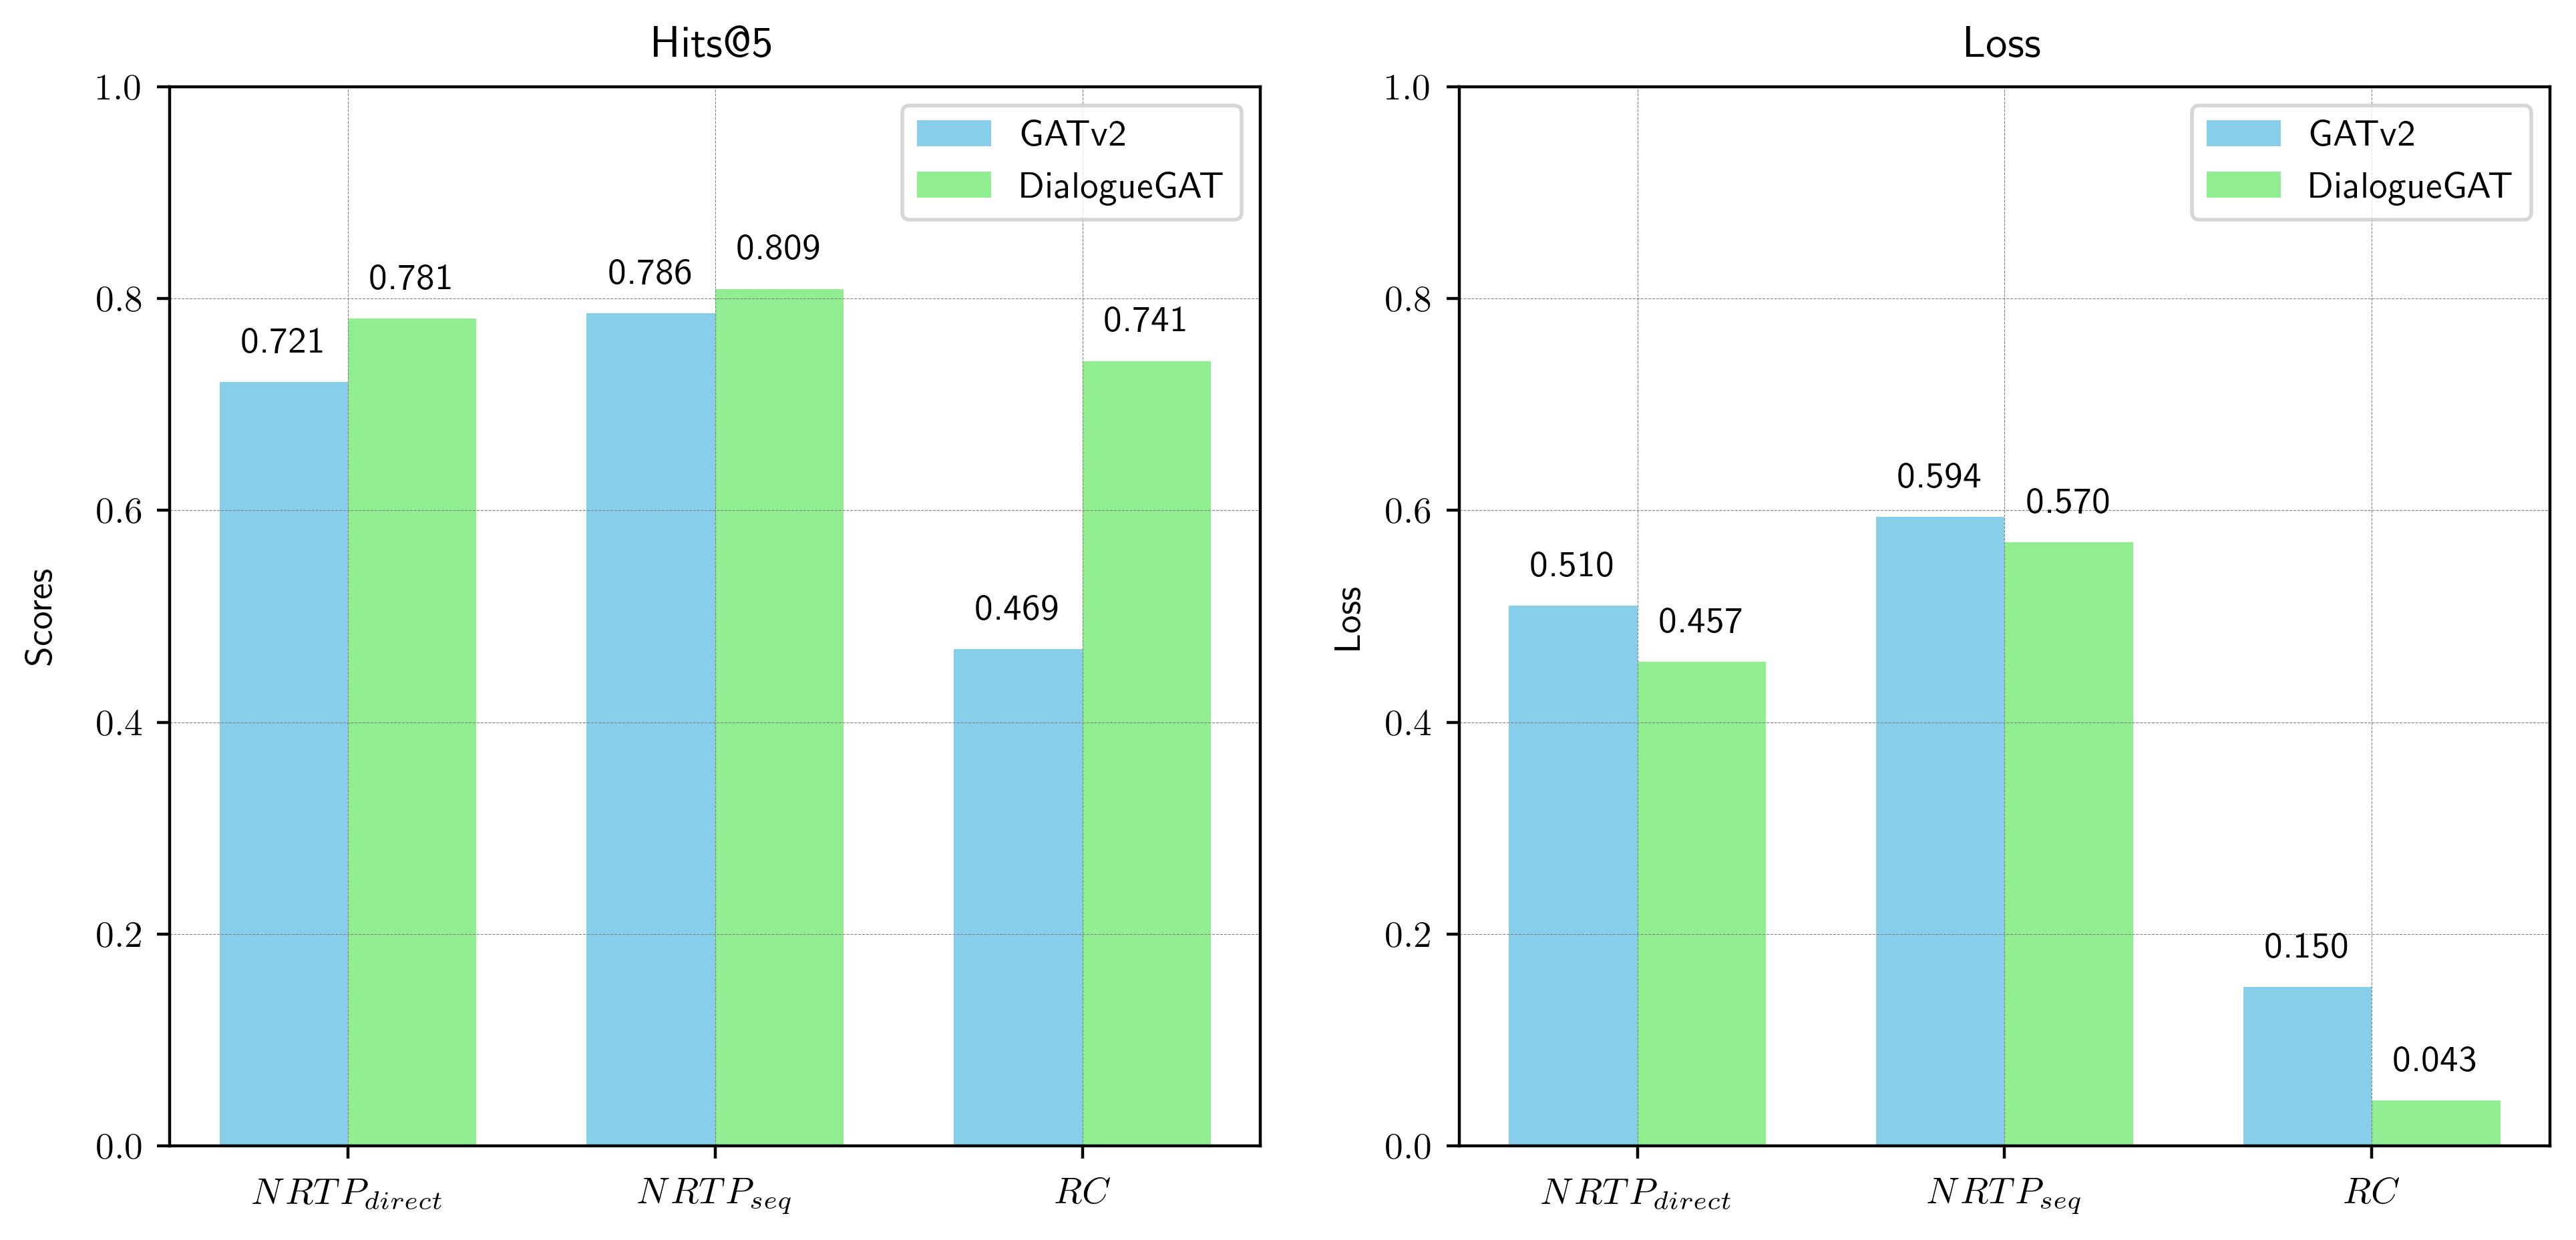
\includegraphics[width=0.5\textwidth]{./images/compare_gatv2_dialoguegat.png}
    \caption{Comparison of GATv2 and DialogueGAT (our proposed) as Dialogue Graph Encoders in Different Tasks. \textit{NRTP} denotes Next Response Type Prediction; \textit{RC} denotes Relations Classification.}
    \label{fig:compare_gatv2_dialoguegat}
\end{figure}

\subsubsection{The Effect of proposed DialogueGAT}
To validate the performance of the proposed DialogueGAT compared with existing GNN methods in Dialogue Graph modeling, we analyze results in the Next Response Type Prediction (NRTP) and Coherence Relations Classification tasks on the validation set. We compare DialogueGAT with GATv2. This comparison is illustrated in Figure \ref{fig:compare_gatv2_dialoguegat}. The experimental results demonstrate that DialogueGAT consistently outperforms GATv2 across all tasks in terms of Hits@5 scores, highlighting its enhanced capability to predict discourse relations (response types) from dialogue context information. Notably, in the Coherence Relations Classification (RC) task, DialogueGAT achieves significant improvements, showcasing its robustness in understanding context relationships. Additionally, the loss metrics further validate the efficiency of DialogueGAT; it registers lower loss values than GATv2 in both NRTP tasks, indicating superior model optimization and better fitting. The most pronounced difference is observed in the RC task, where the loss for DialogueGAT is markedly lower, emphasizing its exceptional performance in accurately classifying coherence relations. These findings suggest that DialogueGAT enhances prediction accuracy and effectively reduces error rates in discourse understanding.

\subsubsection{The Effect of Dialogue Graph Encoder}

\begin{figure}[ht]
    \centering
    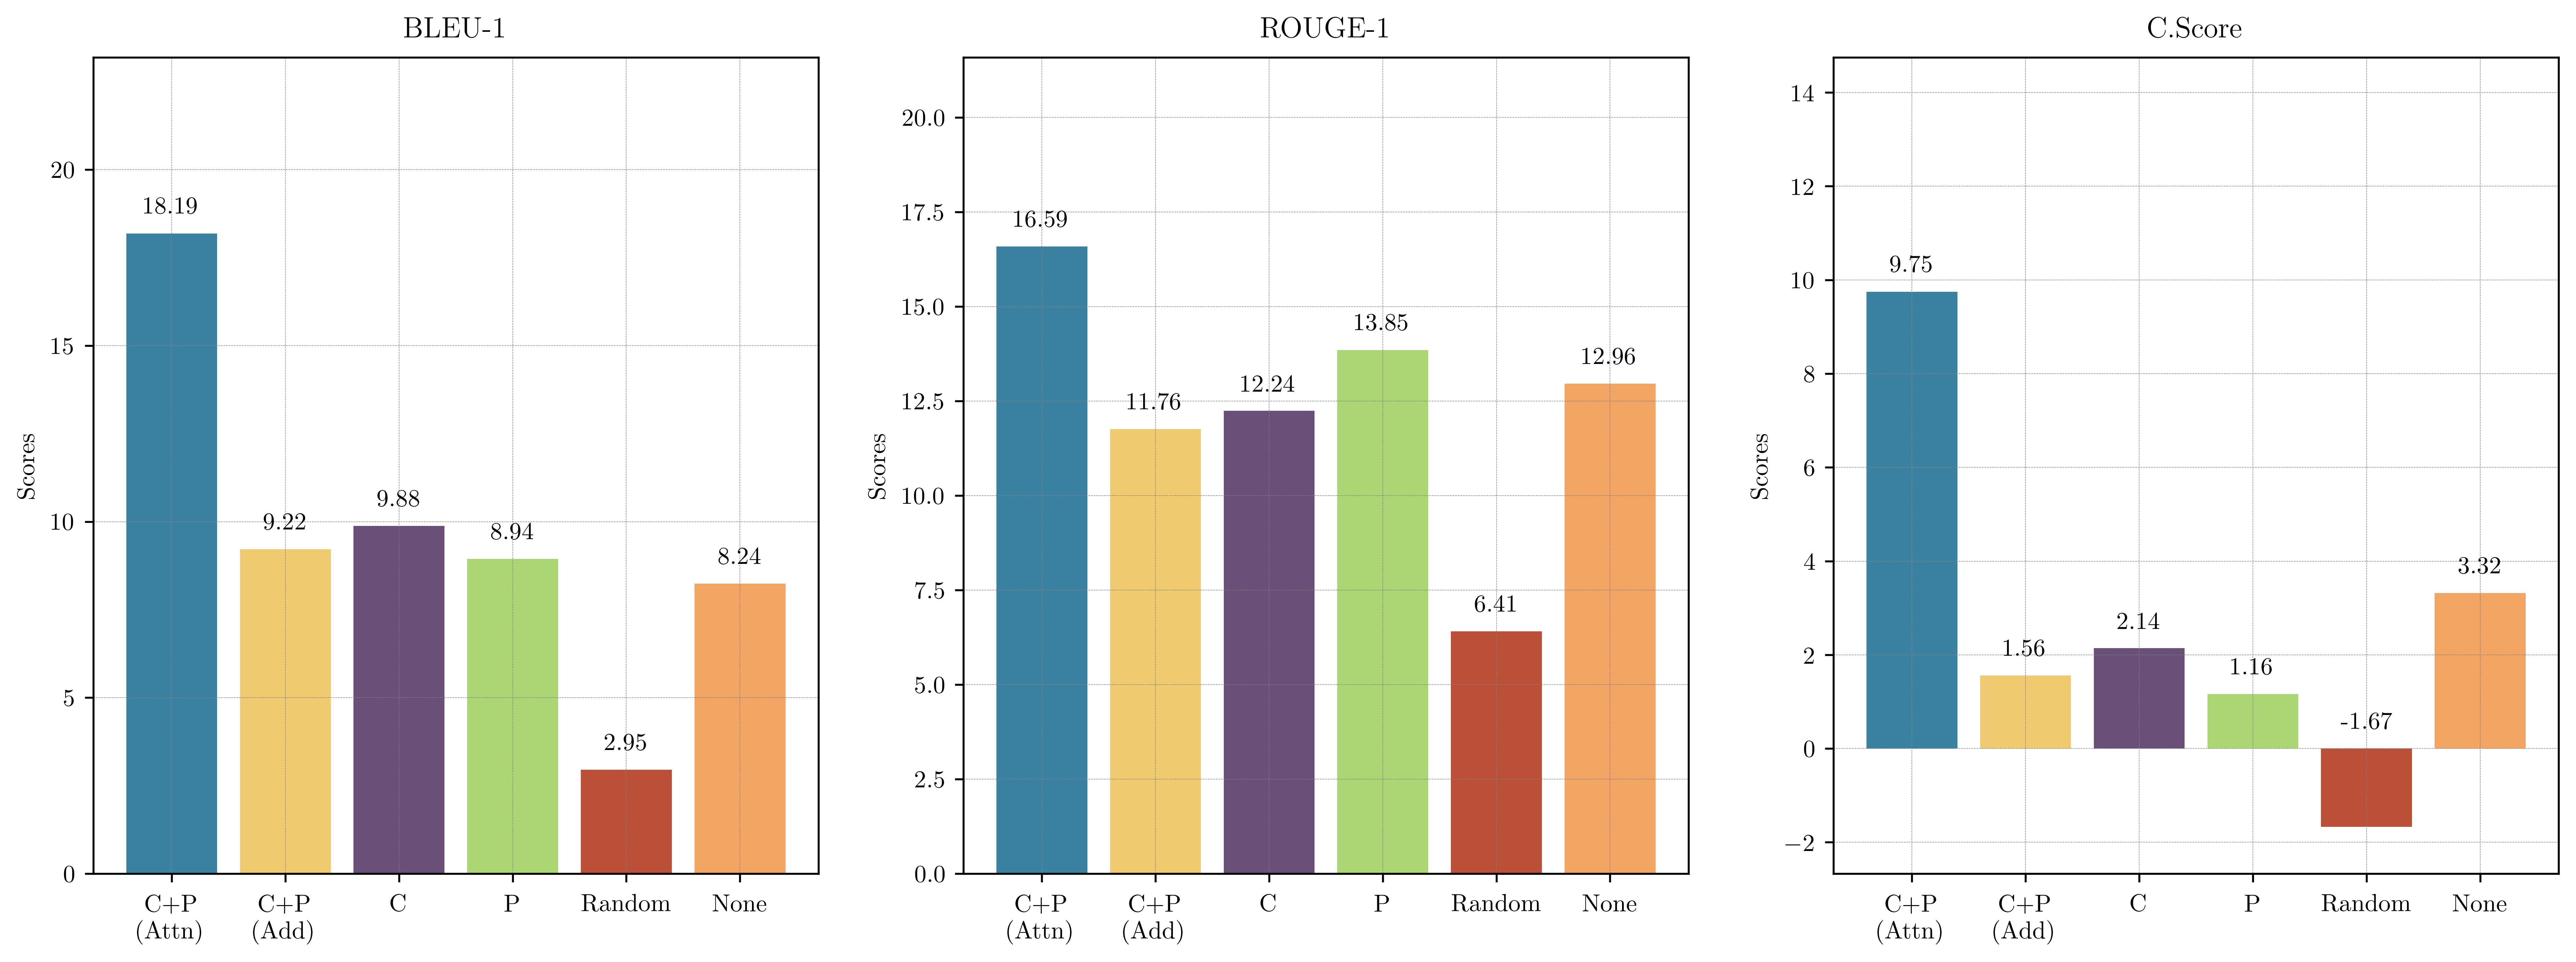
\includegraphics[width=0.5\textwidth]{./images/effectiveness_of_dialogue_graph_encoder.png}
    \caption{Performance analysis of Dialogue Graph Encoder across different settings. Here, "C" represents Context, and "P" represents Persona.}
    \label{fig:effectiveness_of_dialogue_graph_encoder}
\end{figure}

We analyze the effectiveness of the Dialogue Graph Encoder (discussed in Section 3.2.2 fine-tuning phase) under various settings. (1) \textbf{Context+Persona (Attention)}: This is our primary method where we utilize an Attention-based Feature Fusion approach to integrate representations from both the Dialogue Graph and the Persona Graph. (2) \textbf{Context+Persona (Add)}: We replace the Attention-based Feature Fusion approach with a simple addition of the persona and context representations. (3) \textbf{Context}: In this setting, we solely rely on the representation from the Dialogue Graph. (4) \textbf{Persona}: Here, we use only the representation from the Persona Graph. (5) \textbf{Random}: A random vector replaces the output of the Dialogue Graph Encoder. (6) \textbf{None}: The Dialogue Graph Encoder is completely removed from the process, allowing the generator to receive only the context and persona information from the Text Encoder. The comprehensive experimental results can be found in Figure \ref{fig:effectiveness_of_dialogue_graph_encoder}. We report the metrics for BLEU-1, ROUGE-1, and Consistency Score (C.Score).

Our experimental results demonstrate that the attention-based feature fusion approach (Context+Persona (Attention)) significantly outperforms other methods in terms of BLEU-1 and ROUGE-1 scores. These findings confirm that effectively integrating contextual and persona information through an attention mechanism enhances the similarity of the generated responses to the ground-truth responses. In contrast, simpler methods such as addition (Context+Persona (Add)) or those relying solely on context or persona information exhibit lower performance. The scores drastically decrease when random vectors are employed or when the dialogue graph encoder is omitted entirely, which emphasizes the crucial role of structured and meaningful input in producing coherent responses. The consistency scores further elucidate the models' ability to generate responses that align with persona traits. The superior performance of the attention-based method suggests its effectiveness in maintaining persona consistency within the responses. Notably, employing random vectors results in negative C.Score values, indicating that some generated responses are not only irrelevant but also contradictory to the defined personas.

These outcomes reinforce the importance of utilizing attention-based feature fusion in dialogue systems, especially in tasks that require a nuanced understanding of both context and persona. Additionally, the inferior results associated with random inputs and the complete removal of the dialogue graph encoder highlight potential risks of response incoherence and contradiction when inputs are not integrated thoughtfully. We present examples of generated results for these settings in Table \ref{table:case_study_effectiveness_of_dialogue_graph_encoder}.

\subsubsection{The Effect of Tau Values in Dynamic Weighted Aggregation}

\begin{figure}[hb]
    \centering
    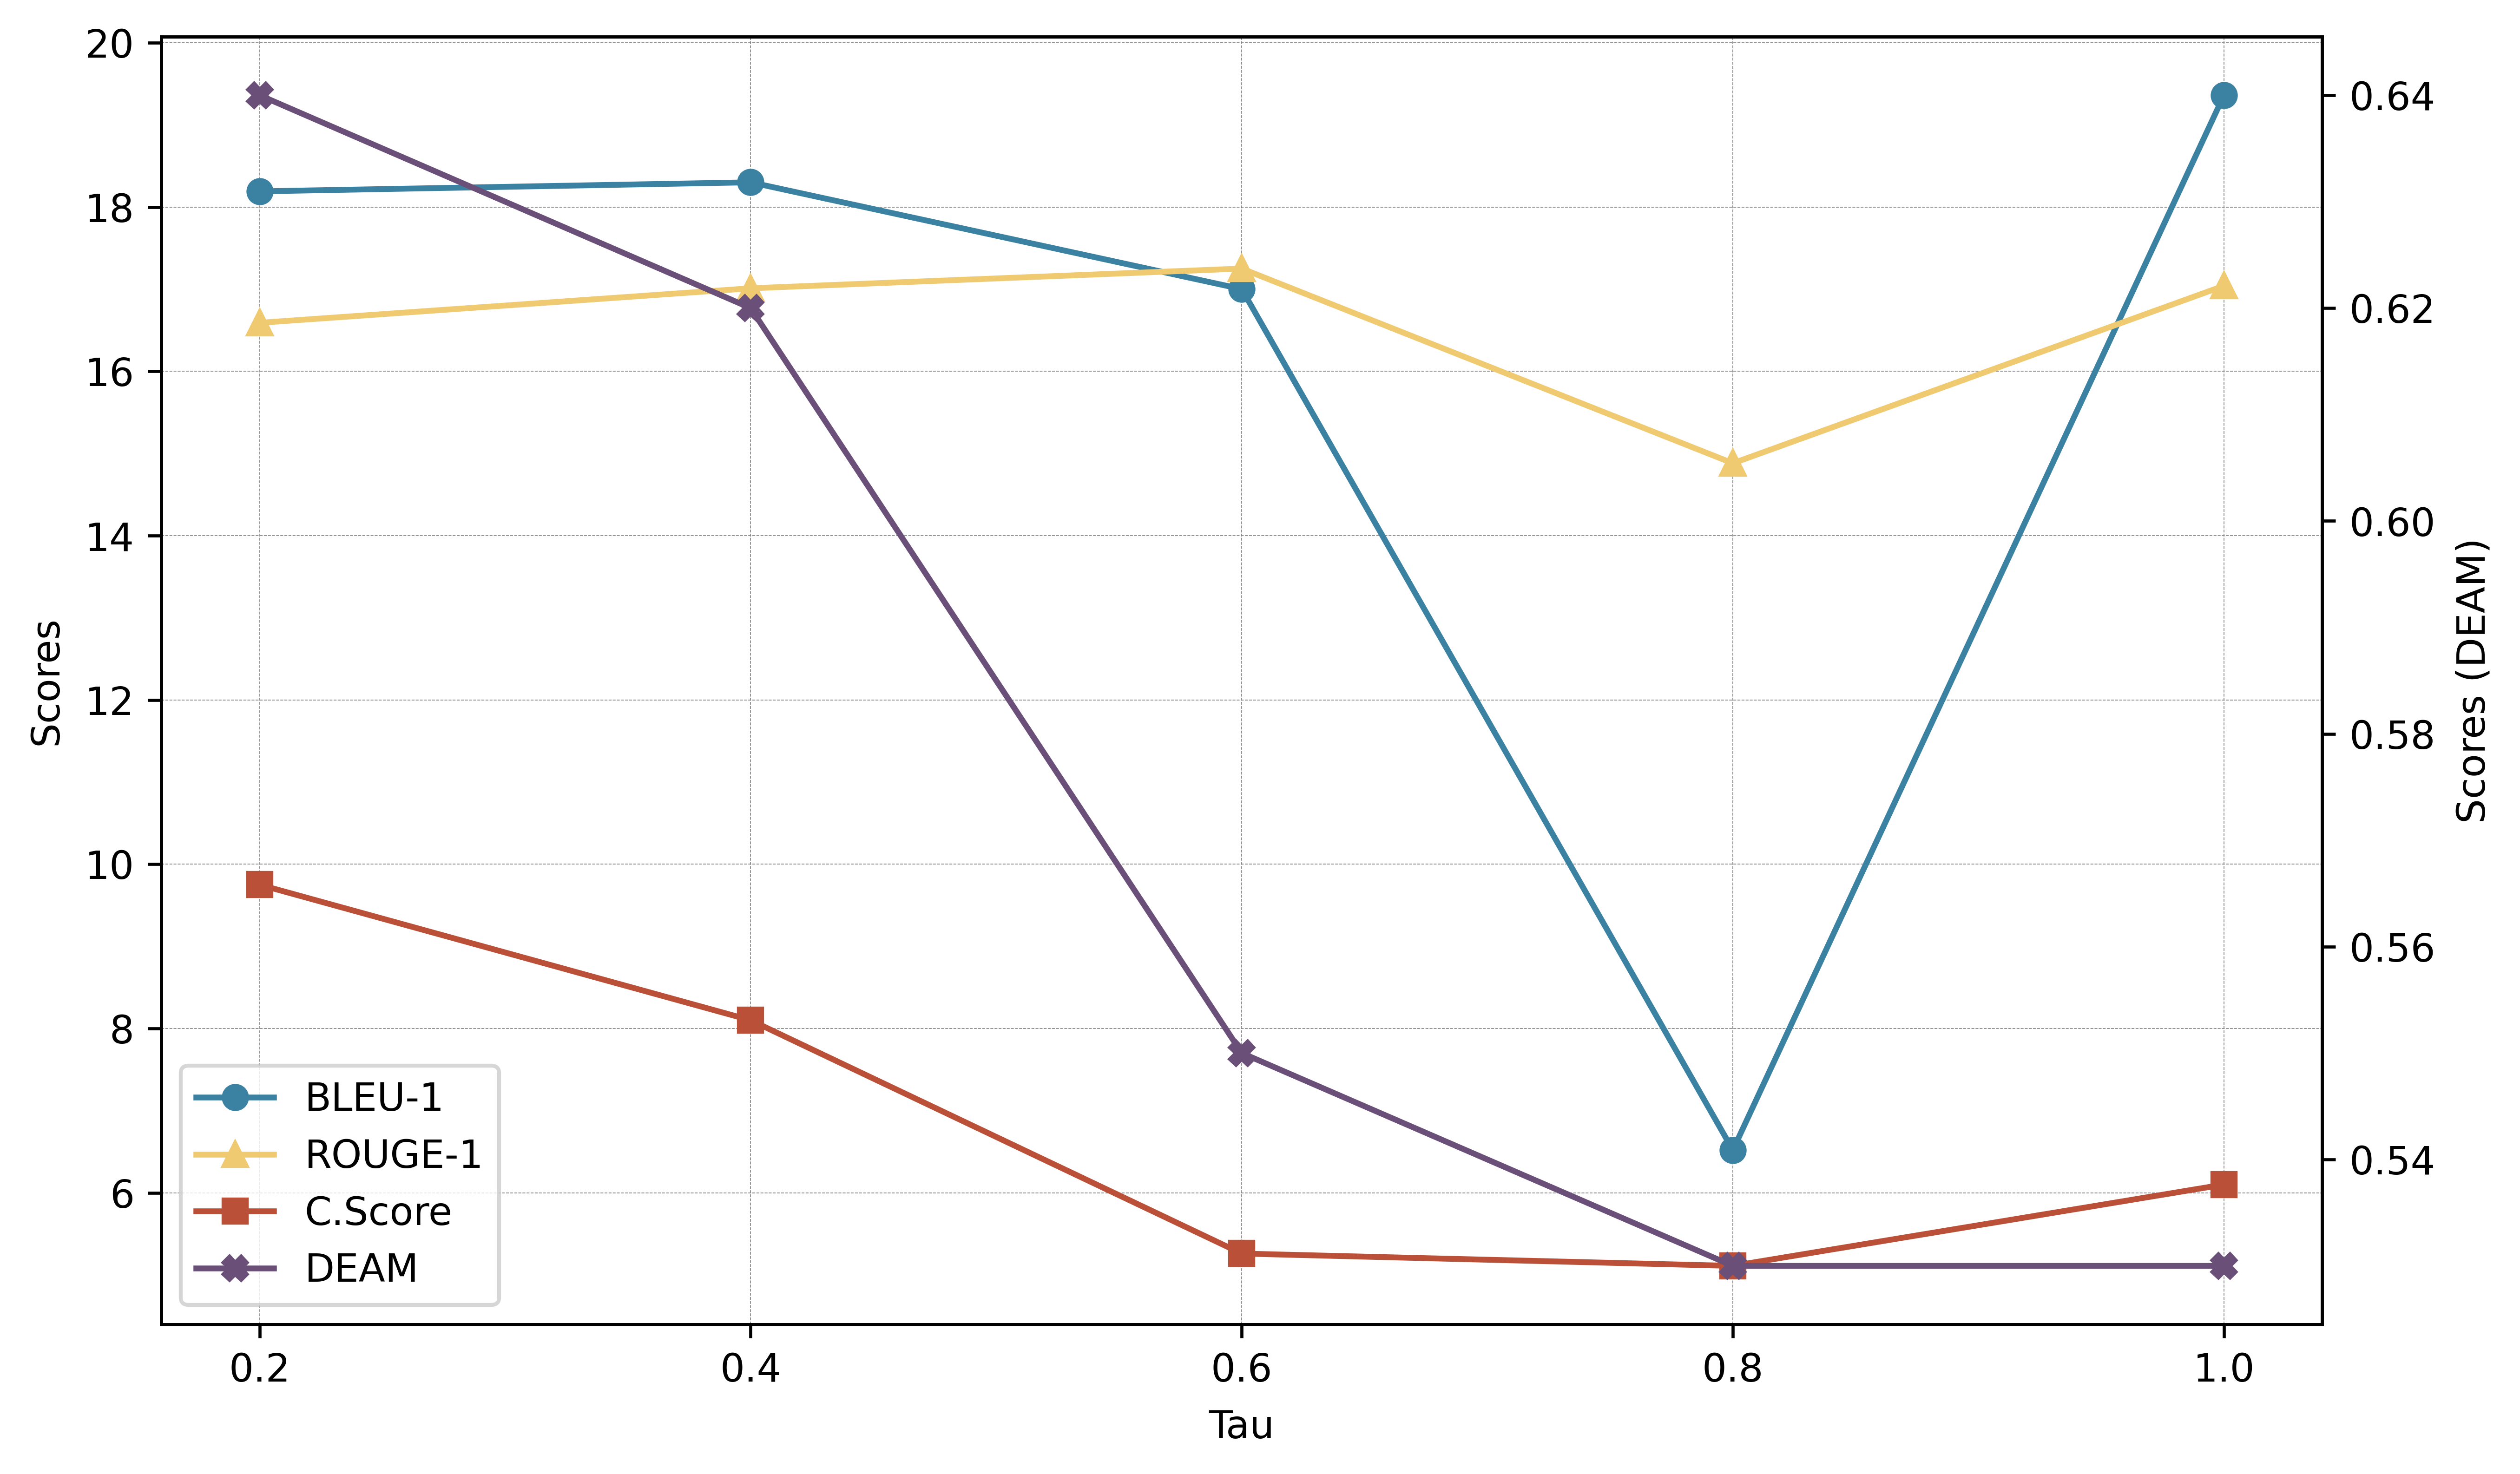
\includegraphics[width=0.5\textwidth]{./images/effectiveness_of_tau_with_deam.png}
    \caption{Performance analysis of $\tau$ in Dynamic Weighted Aggregation.}
    \label{fig:effectiveness_of_tau}
\end{figure}

We analyze the effectiveness of $\tau$ in Dynamic Weighted Aggregation (discussed in Section 3.4). According to our results, shown in Figure \ref{fig:effectiveness_of_tau}, the scores gradually decrease as $\tau$ increases, with the most significant drop occurring at 0.8. Additionally, we observed that the scores, particularly for BLEU-1, actually increase when $\tau$ reaches 1.0. We hypothesize that this is due to our approach, which involves a residual connection (Eq. \ref{eq:dynamic_weighted_aggregation_output}) between the outputs of the Text Encoder and the Dialogue Graph Encoder with the results of the dynamic weighting. When $\tau$ is set to 1.0, it effectively considers only the original outputs, thus retaining a certain level of generative capability. However, this does not enhance persona consistency as much as when $\tau$ is optimally adjusted. This observation confirms that through Dynamic Weighted Aggregation, we can appropriately balance discourse and persona information.


\begin{table*}[ht]
\centering
\def\arraystretch{1.2}%
\begin{tabular}{|p{3.5cm}|p{12cm}|}

\hline
\rowcolor{yellow}
\multicolumn{2}{|c|}{\textbf{Persona}} \\
\hline
\multicolumn{2}{|l|}{I have two dogs.} \\
\multicolumn{2}{|l|}{I like to work on vintage cars.} \\
\multicolumn{2}{|l|}{My favorite music is country.} \\
\multicolumn{2}{|l|}{I own two vintage mustangs.} \\
\hline

\rowcolor{yellow}
\multicolumn{2}{|c|}{\textbf{Context}} \\
\hline
\multicolumn{2}{|l|}{Q: Hi! How are you doing tonight?} \\
\multicolumn{2}{|l|}{R: I'm doing great. Just relaxing with my two dogs.} \\
\multicolumn{2}{|l|}{Q: Great. In my spare time I do volunteer work.} \\
\multicolumn{2}{|l|}{R: That's neat. What kind of volunteer work do you do?} \\
\multicolumn{2}{|l|}{Q: I work in a homeless shelter in my town.} \\
\multicolumn{2}{|l|}{R: Good for you. Do you like vintage cars? I've two older mustangs.} \\
\multicolumn{2}{|l|}{Q: Cool. Not really into cars. My day job is wrestling.} \\
\multicolumn{2}{|l|}{R: Cars are my thing. Vintage cars. I love working on them. Wrestling? Do you enjoy it?} \\
\multicolumn{2}{|l|}{Q: Yes, I love the crowds, getting to know people.} \\
\multicolumn{2}{|l|}{R: I didn't think about the crowd aspect of wrestling. I do not like crowds.} \\
\multicolumn{2}{|l|}{Q: Understood. When I need to be alone, I work out a few times each week.} \\
\multicolumn{2}{|l|}{R: I agree. Working out is a great way to burn off steam. Do you like country music?} \\
\hline

\rowcolor{yellow}
\multicolumn{2}{|c|}{\textbf{Query}} \\
\hline
\multicolumn{2}{|l|}{A little bit. I can get into taylor swift.} \\

\hhline{|==|}
\rowcolor[RGB]{204,217,245}
\multicolumn{2}{|c|}{\textbf{Response}} \\
\hhline{|==|}
\textbf{Context+Persona (Attention)} & I do not like her. She's a bit too uptight for my taste. But I like her music. \\
\textbf{Context+Persona (Add)} & I can get may may and m and may and j on for more of her \\
\textbf{Context} &  What was she like? \\
\textbf{Persona} & I like country music too. \\
\textbf{Random} & you The A’ A A played The old White lead A Barbara at The The 17… \\
\textbf{None} & I like country music as well. \\

\hline
\end{tabular}
\caption{Case analysis of the effectiveness of Dialogue Graph Encoder.}
\label{table:case_study_effectiveness_of_dialogue_graph_encoder}
\end{table*}

\subsection{Case Study}
Teable \ref{table:case_study_1}, \ref{table:case_study_2}, \ref{table:case_study_3}, and \ref{table:case_study_4} present the personalized responses generated by various methods using the ConvAI2 dataset. The responses generated by the proposed method, \textbf{MUDI}, demonstrated greater consistency with their respective personas and showed higher coherence with both the context and the query, appearing more human-like. As illustrated in Table \ref{table:case_study_1}, the responses from BoB were incoherent with the query, though they remained consistent with the persona. PAA often overfocused on the persona, leading to repetitive narratives of the persona description. Both LMEDR and our model produced responses that were more coherent, basing them on the user persona, but MUDI was able to generate more detailed replies, such as adding personal aspirations to the basic response about family support. 

In Table \ref{table:case_study_2}, the responses generated by BoB were irrelevant to the personas and incoherent with the context. PAA exhibited a global incoherence from the dialogue context, failing to maintain a logical flow in the conversation. While LMEDR generated a somewhat relevant response indicating a dream car, it lacked depth and personal context. On the other hand, MUDI produced a more personalized and contextually rich response that not only mentions the dream car but also integrates family dynamics, demonstrating a deeper understanding of the persona's background and the complexities in their personal relationships. 

In Table \ref{table:case_study_3}, BoB and PAA tended to overlook content from the ongoing dialogue, generating repetitive responses that rendered the entire conversation incoherent. Although LMEDR was able to generate adequate responses, our model excelled by producing more natural responses through the inclusion of responsive questions. 

As shown in Table \ref{table:case_study_4}, BoB diverged from the persona's preference by mentioning classic rock instead of country music, showing a misalignment with the user’s interests. LMEDR and PAA both correctly identified and responded with a generic appreciation for country music, aligning with the persona’s interests, yet their responses lacked specific engagement with the user’s mention of Taylor Swift or deeper personal nuances. MUDI's response, while initially not favoring Taylor Swift, cleverly circled back to acknowledge her music, demonstrating not only a nuanced understanding of the persona's tastes but also adding an interesting twist to the conversation. This illustrates MUDI's ability to generate engaging and lifelike responses, making the interaction more intriguing for users.

In summary, our model \textbf{MUDI} effectively combines dialogue and persona elements to generate appropriate responses. Furthermore, it excels at using responsive questions to enhance the conversation's naturalness.


% ----------------------------------------------
% Case Study 1
% ----------------------------------------------

\begin{table*}[ht]
\centering
\def\arraystretch{1.2}%
\begin{tabular}{|l|p{11cm}|}

\hline
\rowcolor{yellow}
\multicolumn{2}{|c|}{\textbf{Persona}} \\
\hline
\multicolumn{2}{|l|}{My dream car is a rolls royce ghost.} \\
\multicolumn{2}{|l|}{I currently work for a watch dealer.} \\
\multicolumn{2}{|l|}{My family does not support my career choices.} \\
\multicolumn{2}{|l|}{I often shop for shoes and watches.} \\
\multicolumn{2}{|l|}{I like shopping.} \\
\hline

\rowcolor{yellow}
\multicolumn{2}{|c|}{\textbf{Context}} \\
\hline
\multicolumn{2}{|l|}{Q: Good evening. What are you up to?} \\
\multicolumn{2}{|l|}{R: Hello, how are you ? I am well. I like to shop for shoes and watches.} \\
\multicolumn{2}{|l|}{Q: I don't shop much. Prefer to relax at home with my cow.} \\
\multicolumn{2}{|l|}{R: What do you do ? I'm work for a watch dealer.} \\
\hline

\rowcolor{yellow}
\multicolumn{2}{|c|}{\textbf{Query}} \\
\hline
\multicolumn{2}{|l|}{No wonder you like watches ! I'm a commercial electrician.} \\

\hhline{|==|}
\rowcolor[RGB]{204,217,245}
\multicolumn{2}{|c|}{\textbf{Response}} \\
\hhline{|==|}
\textbf{GOLD} & wonderful! yeah, however, my family does not support my choice of career. \\
\textbf{BoB} & I work at a dealership, but I am not very good at it. \\
% \textbf{P$^2$BOT} & what do you do for a living ? i work for the watch. \\
\textbf{LMEDR} & My family does not support my career choices. \\
\textbf{PAA} & I like to shop. I also like to shop. \\
\textbf{MUDI} & My family does not support my career choices. I want to drive a rolls royce ghost. \\

\hline
\end{tabular}
\caption{Case analysis of personalized response generation on the ConvAI2 dataset.}
\label{table:case_study_1}
\end{table*}

% ----------------------------------------------
% Case Study 2
% ----------------------------------------------

\begin{table*}[ht]
\centering
\def\arraystretch{1.2}%
\begin{tabular}{|l|p{11cm}|}

\hline
\rowcolor{yellow}
\multicolumn{2}{|c|}{\textbf{Persona}} \\
\hline
\multicolumn{2}{|l|}{My dream car is a rolls royce ghost.} \\
\multicolumn{2}{|l|}{I currently work for a watch dealer.} \\
\multicolumn{2}{|l|}{My family does not support my career choices.} \\
\multicolumn{2}{|l|}{I often shop for shoes and watches.} \\
\multicolumn{2}{|l|}{I like shopping.} \\
\hline

\rowcolor{yellow}
\multicolumn{2}{|c|}{\textbf{Context}} \\
\hline
\multicolumn{2}{|l|}{Q: Good evening. What are you up to?} \\
\multicolumn{2}{|l|}{R: Hello, how are you ? I am well. I like to shop for shoes and watches.} \\
\multicolumn{2}{|l|}{Q: I don't shop much. Prefer to relax at home with my cow.} \\
\multicolumn{2}{|l|}{R: What do you do ? I'm work for a watch dealer.} \\
\multicolumn{2}{|l|}{Q: No wonder you like watches! I'm a commercial electrician.} \\
\multicolumn{2}{|l|}{R: Wonderful! Yeah, however, my family does not support my choice of career.} \\
\hline

\rowcolor{yellow}
\multicolumn{2}{|c|}{\textbf{Query}} \\
\hline
\multicolumn{2}{|l|}{Why not? Family is important.} \\

\hhline{|==|}
\rowcolor[RGB]{204,217,245}
\multicolumn{2}{|c|}{\textbf{Response}} \\
\hhline{|==|}
\textbf{GOLD} & I'm not sure why they do not. Do you like cars? \\
\textbf{BoB} & I am not sure. I am a watch dealer. \\
% \textbf{P$^2$BOT} & my family doesn't support my lifestyle choices. \\
\textbf{LMEDR} & I do not know. I do have a dream car though. It is a rolls royce ghost. \\
\textbf{PAA} & I am a watch dealer. I have a lot of money. \\
\textbf{MUDI} & yes agree! I want to drive a rolls royce ghost car, but my family does not like that. \\

\hline
\end{tabular}
\caption{Case analysis of personalized response generation on the ConvAI2 dataset.}
\label{table:case_study_2}
\end{table*}

% ----------------------------------------------
% Case Study 3
% ----------------------------------------------

\begin{table*}[ht]
\centering
\def\arraystretch{1.2}%
\begin{tabular}{|l|p{11cm}|}

\hline
\rowcolor{yellow}
\multicolumn{2}{|c|}{\textbf{Persona}} \\
\hline
\multicolumn{2}{|l|}{I listen to rap music.} \\
\multicolumn{2}{|l|}{I produce music for artists.} \\
\multicolumn{2}{|l|}{I drive a 2015 Honda Civic.} \\
\multicolumn{2}{|l|}{My favorite food is pizza.} \\
\hline

\rowcolor{yellow}
\multicolumn{2}{|c|}{\textbf{Context}} \\
\hline
\multicolumn{2}{|l|}{Q: Hi, how are you? Do you have any brothers or sisters?} \\
\multicolumn{2}{|l|}{R: No I don't do you?} \\
\multicolumn{2}{|l|}{Q: Yes, I'm 13 and I've an older brother.} \\
\multicolumn{2}{|l|}{R: That's nice what kind of music do you like.} \\
\multicolumn{2}{|l|}{Q: I do not have much time as I play soccer. You?} \\
\multicolumn{2}{|l|}{R: I am a music producer for rap artists} \\
\hline

\rowcolor{yellow}
\multicolumn{2}{|c|}{\textbf{Query}} \\
\hline
\multicolumn{2}{|l|}{Cool I like rap. I hate maths though! Do you have other hobbies?} \\

\hhline{|==|}
\rowcolor[RGB]{204,217,245}
\multicolumn{2}{|c|}{\textbf{Response}} \\
\hhline{|==|}
\textbf{GOLD} & Work takes up a lot of my time. \\
\textbf{BoB} & I like music and I like to listen to music. \\
% \textbf{P$^2$BOT} & I like to listen to rap music. \\
\textbf{LMEDR} & I like to drive my honda civic. \\
\textbf{PAA} & I like rap music, I produce it for artists. \\
\textbf{MUDI} & I like to go my old Honda Civic car and eat pizza. Do you have any hobbies? \\

\hline
\end{tabular}
\caption{Case analysis of personalized response generation on the ConvAI2 dataset.}
\label{table:case_study_3}
\end{table*}

% ----------------------------------------------
% Case Study 4
% ----------------------------------------------

\begin{table*}[ht]
\centering
\def\arraystretch{1.2}%
\begin{tabular}{|l|p{11cm}|}

\hline
\rowcolor{yellow}
\multicolumn{2}{|c|}{\textbf{Persona}} \\
\hline
\multicolumn{2}{|l|}{I have two dogs.} \\
\multicolumn{2}{|l|}{I like to work on vintage cars.} \\
\multicolumn{2}{|l|}{My favorite music is country.} \\
\multicolumn{2}{|l|}{I own two vintage mustangs.} \\
\hline

\rowcolor{yellow}
\multicolumn{2}{|c|}{\textbf{Context}} \\
\hline
\multicolumn{2}{|l|}{Q: Hi! How are you doing tonight?} \\
\multicolumn{2}{|l|}{R: I'm doing great. Just relaxing with my two dogs.} \\
\multicolumn{2}{|l|}{Q: Great. In my spare time I do volunteer work.} \\
\multicolumn{2}{|l|}{R: That's neat. What kind of volunteer work do you do?} \\
\multicolumn{2}{|l|}{Q: I work in a homeless shelter in my town.} \\
\multicolumn{2}{|l|}{R: Good for you. Do you like vintage cars? I've two older mustangs.} \\
\multicolumn{2}{|l|}{Q: Cool. Not really into cars. My day job is wrestling.} \\
\multicolumn{2}{|l|}{R: Cars are my thing. Vintage cars. I love working on them. Wrestling? Do you enjoy it?} \\
\multicolumn{2}{|l|}{Q: Yes, I love the crowds, getting to know people.} \\
\multicolumn{2}{|l|}{R: I didn't think about the crowd aspect of wrestling. I do not like crowds.} \\
\multicolumn{2}{|l|}{Q: Understood. When I need to be alone, I work out a few times each week.} \\
\multicolumn{2}{|l|}{R: I agree. Working out is a great way to burn off steam. Do you like country music?} \\
\hline

\rowcolor{yellow}
\multicolumn{2}{|c|}{\textbf{Query}} \\
\hline
\multicolumn{2}{|l|}{A little bit. I can get into taylor swift.} \\

\hhline{|==|}
\rowcolor[RGB]{204,217,245}
\multicolumn{2}{|c|}{\textbf{Response}} \\
\hhline{|==|}
\textbf{GOLD} & lol. She's more pop now. Her old stuff was country. I like classic country. \\
\textbf{BoB} & I'm not much into music. I like classic rock. \\
% \textbf{P$^2$BOT} &  \\
\textbf{LMEDR} & Yes, I love country music. \\
\textbf{PAA} & I do. I love to listen to country music. \\
\textbf{MUDI} & I do not like her. She's a bit too uptight for my taste. But I like her music. \\

\hline
\end{tabular}
\caption{Case analysis of personalized response generation on the ConvAI2 dataset.}
\label{table:case_study_4}
\end{table*}


\end{document}
